\subsection{Comparison of Pathfinding Algorithms}

\begin{table}[h]
    \centering
    \begin{tabular}{|c|c|c|c|c|c|}
        \hline
        \textbf{Algorithm} & \textbf{Steps} & \textbf{Weight} & \textbf{Nodes Explored} & \textbf{Time (ms)} & \textbf{Memory} \\
        \hline
        BFS & \textbf{16} & 695 & 5327 & 480.75 & 3.01 MB \\
        \hline
        DFS & 85 & 707 & 444 & 57.66 & 222.34 KB \\
        \hline
        UCS & 24 & \textbf{405} & 20404 & 1560.00 & 13.04 MB \\
        \hline
        A* & 24 & \textbf{405} & 2146 & 382.55 & 1.92 MB \\
        \hline
        GBFS & 26 & \textbf{405} & \textbf{99} & \textbf{16.15} & \textbf{82.50 KB} \\
        \hline
        Dijkstra & 24 & \textbf{405} & 29450 & 2040.00 & 18.28 MB \\
        \hline
    \end{tabular}
    \label{tab:sokoban_comparison}
\end{table}

\begin{figure}[H]
    \centering
    \begin{subfigure}{0.46\textwidth}
        \centering
        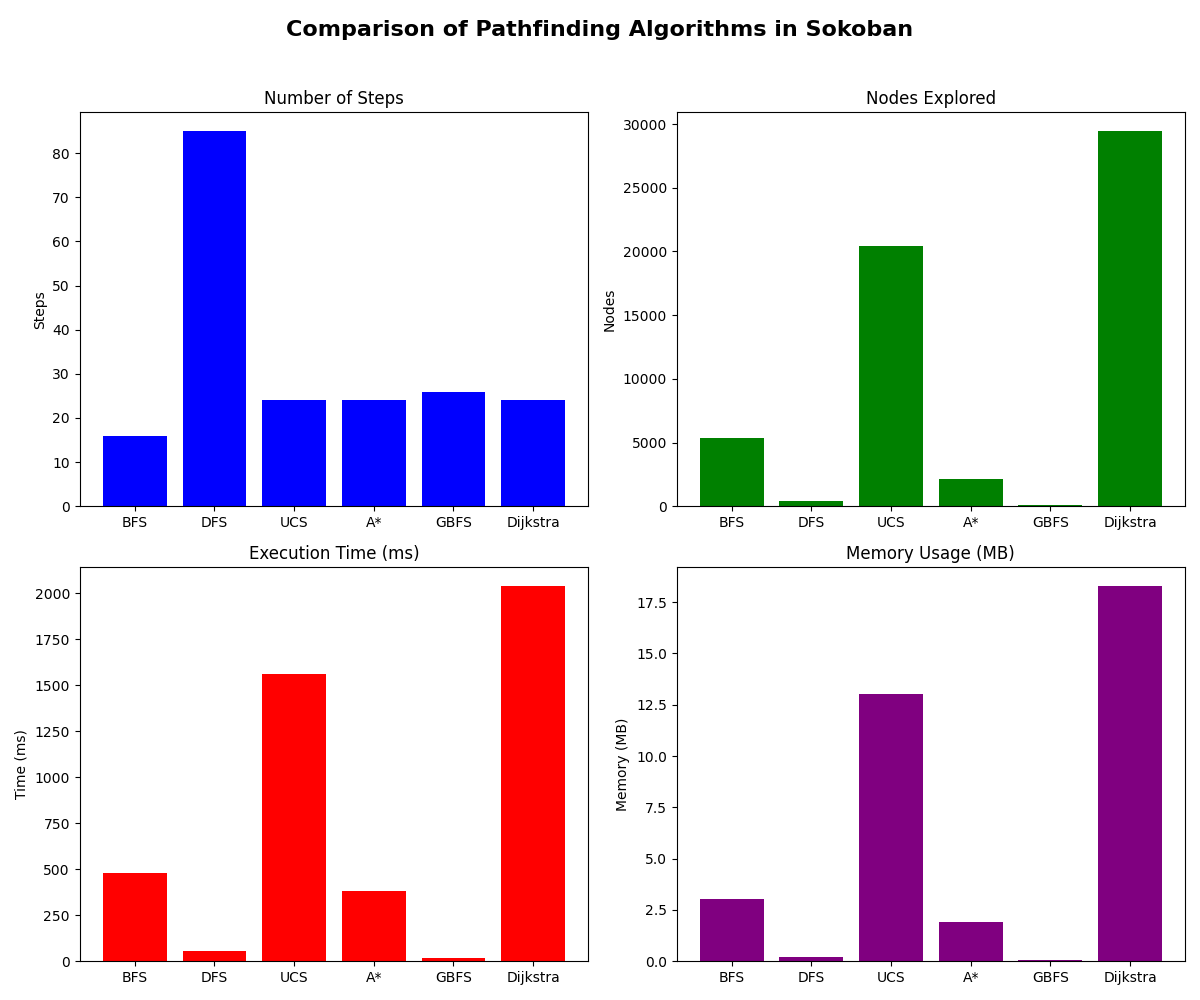
\includegraphics[width=0.9\textwidth]{imgs/test1.png}
        \caption{Test 1}
    \end{subfigure}
    \hfill
    \begin{subfigure}{0.46\textwidth}
        \centering
        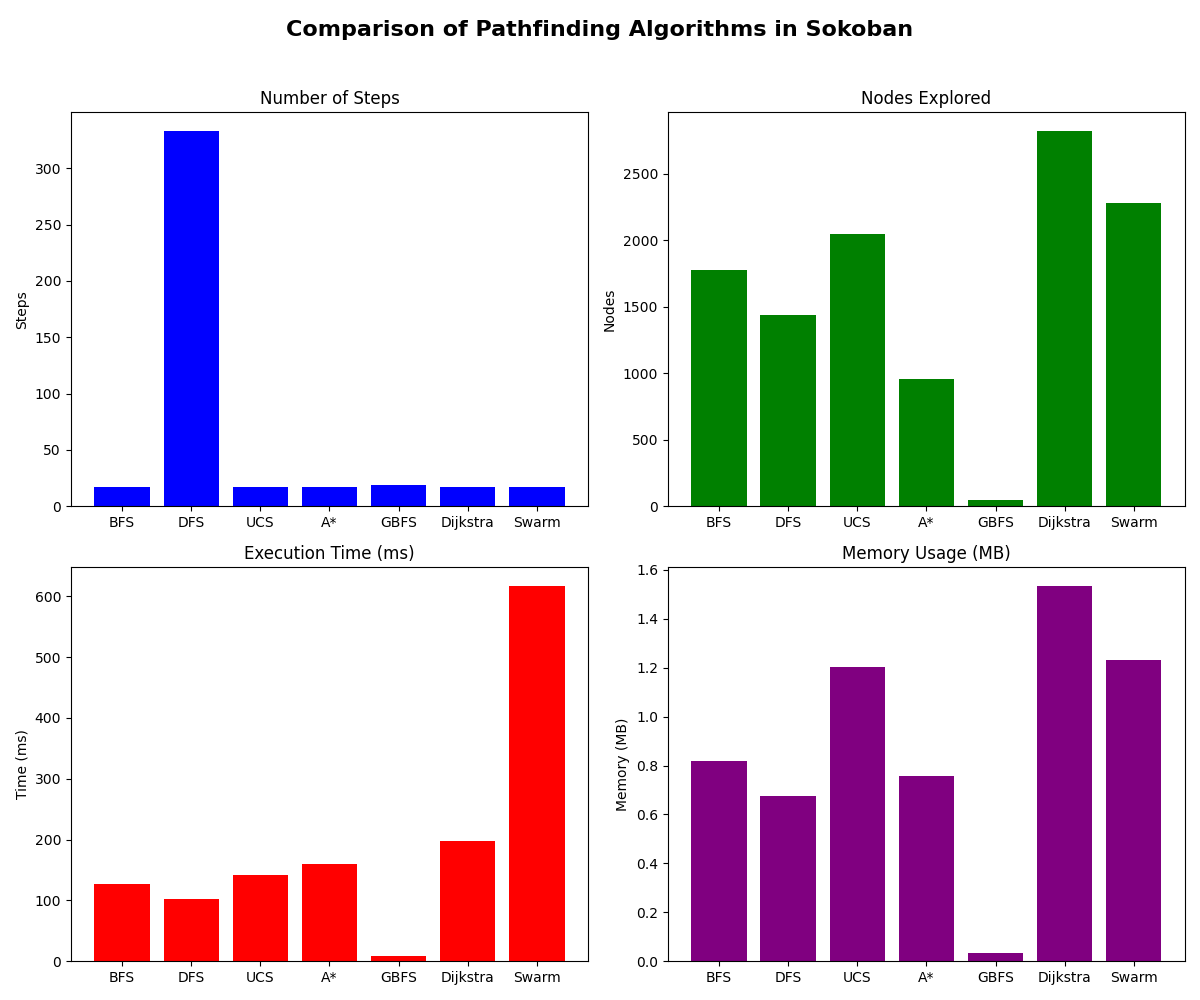
\includegraphics[width=0.9\textwidth]{imgs/test6.png}
        \caption{Test 6}
    \end{subfigure}
    \vfill
    \begin{subfigure}{0.46\textwidth}
        \centering
        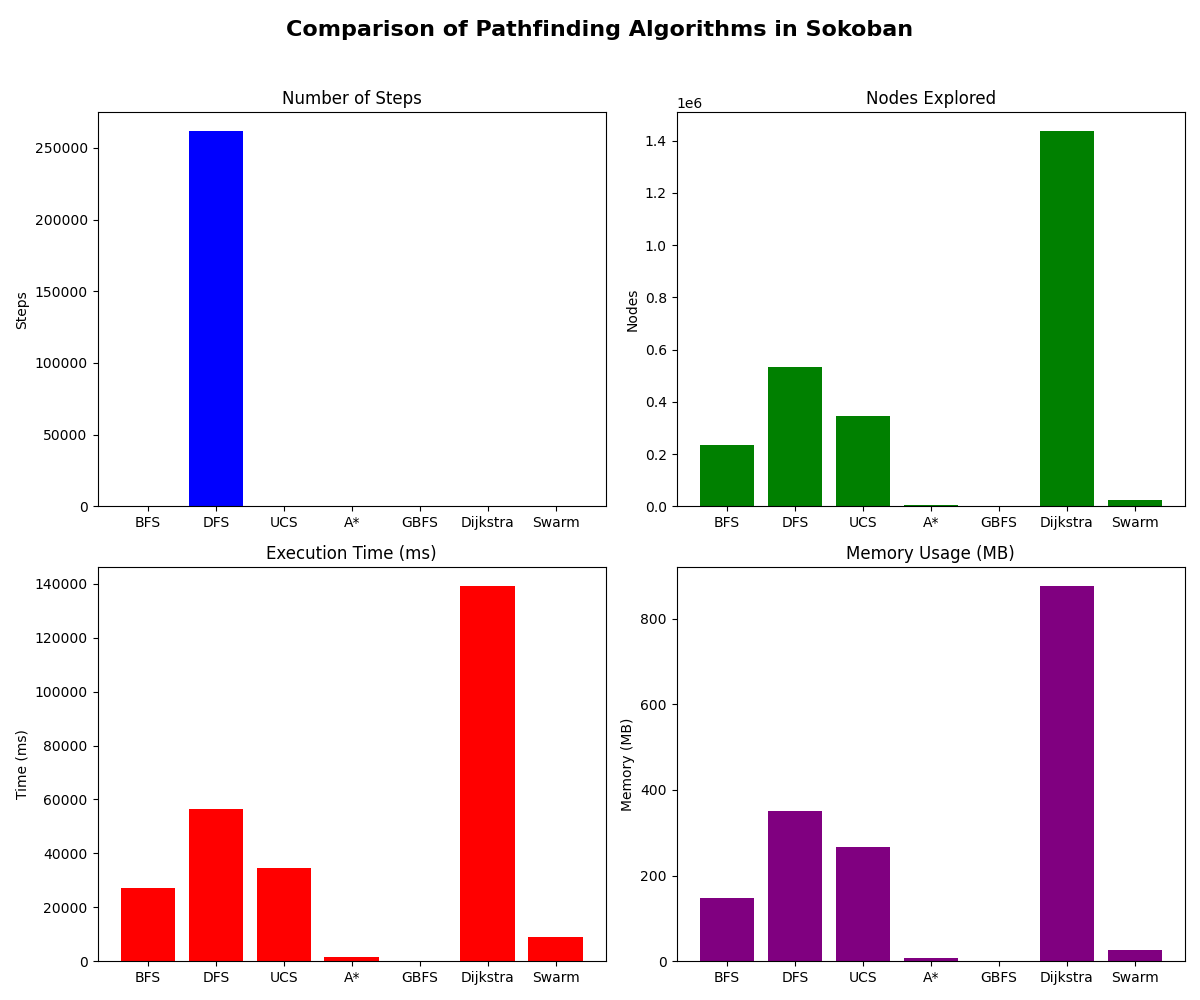
\includegraphics[width=0.9\textwidth]{imgs/test22.png}
        \caption{Test 22}
    \end{subfigure}
    \hfill
    \begin{subfigure}{0.46\textwidth}
        \centering
        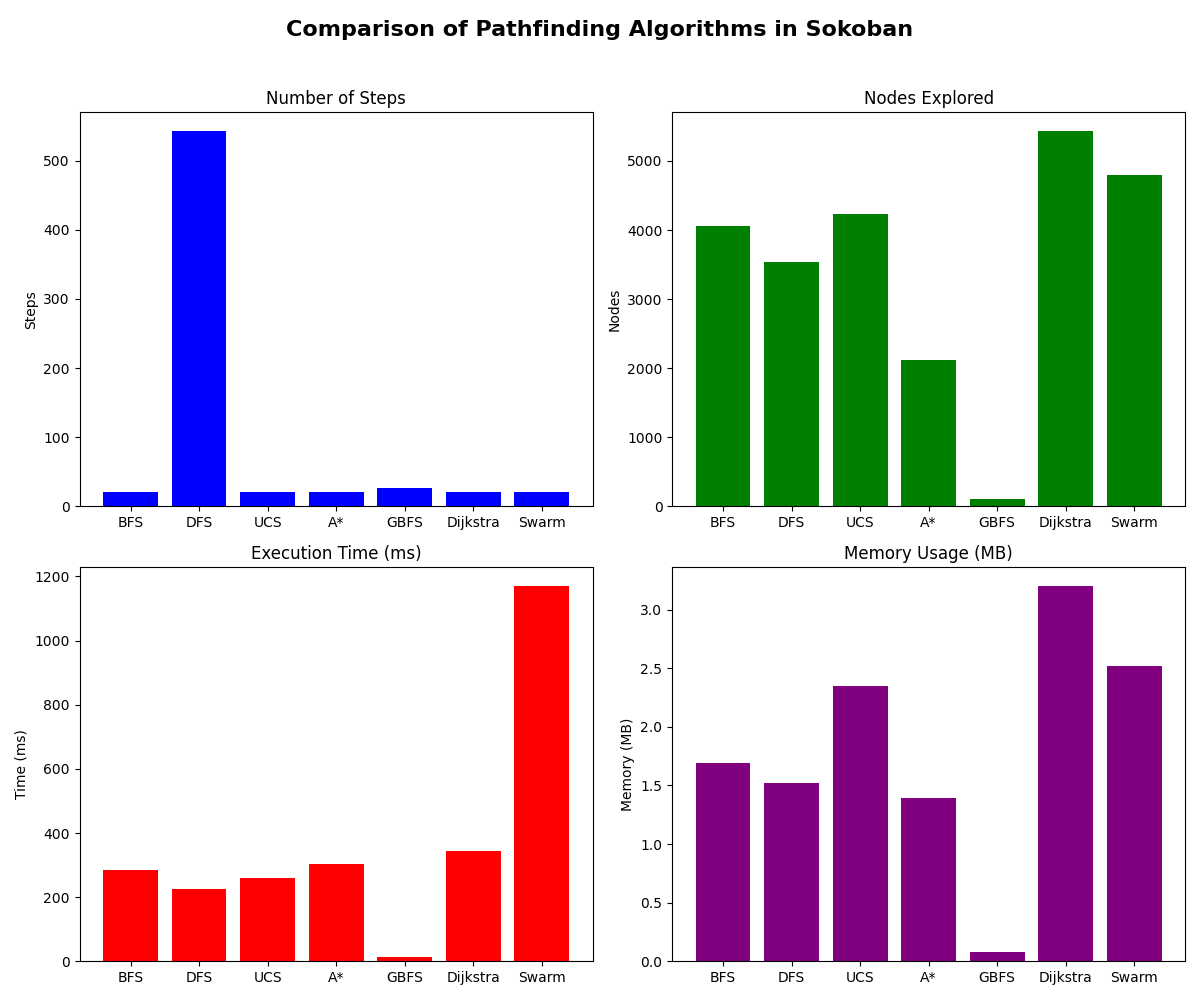
\includegraphics[width=0.9\textwidth]{imgs/test24.png}
        \caption{Test 24}
    \end{subfigure}
    \caption{Performance Comparison of Pathfinding Algorithms}
    \label{fig:comparison}
\end{figure}


\subsubsection{Conclusion}
\noindent This report analyzed various search algorithms applied to the Sokoban problem, comparing their efficiency in terms of steps taken, nodes expanded, time, and memory usage. The results indicate that:
\begin{itemize}
    \item \textbf{A*} and \textbf{UCS} produced optimal solutions but required significant memory and processing time.
    \item \textbf{BFS} efficiently found the shortest path in unweighted space but struggled in large graphs.
    \item \textbf{DFS} explored deeply but was inefficient for finding optimal paths.
    \item \textbf{GBFS} was the fastest algorithm but sometimes produced suboptimal solutions due to its greedy nature.
    \item \textbf{Dijkstra’s} algorithm performed similarly to UCS but expanded more nodes due to its exhaustive nature.
    \item \textbf{Swarm-based approaches} showed potential in parallelized exploration, though their performance depends heavily on heuristic design.
\end{itemize}
Future improvements could involve enhanced heuristics, hybrid approaches, or reinforcement learning techniques to further optimize search performance in Sokoban and similar problems.